\documentclass{article}
\usepackage{tikz}
\begin{document}
\begin{center}
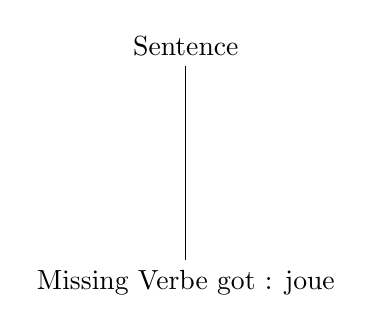
\begin{tikzpicture}
\node{Sentence}[sibling distance = 3cm, level distance = 3cm, align=center]
child {node {Missing Verbe got : joue}};
\end{tikzpicture}
\end{center}
\begin{center}
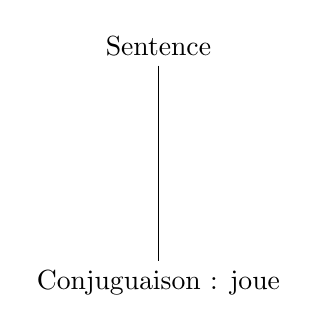
\begin{tikzpicture}
\node{Sentence}[sibling distance = 3cm, level distance = 3cm, align=center]
child {node {Conjuguaison : joue}};
\end{tikzpicture}
\end{center}
\begin{center}
\begin{tikzpicture}
\node{Sentence}[sibling distance = 3cm, level distance = 3cm, align=center]
child { node {GV \\ O3, m, s} child { node {Sujet \\ O3, m, s} child { node {Pronom\_sujet \\ O3, m, s} child {node {il}}}}child { node {Verbe \\ i, t, n, q, \_, \_, a, Ip,Sp, 3s} child {node {joue}}}};
\end{tikzpicture}
\end{center}
\begin{center}
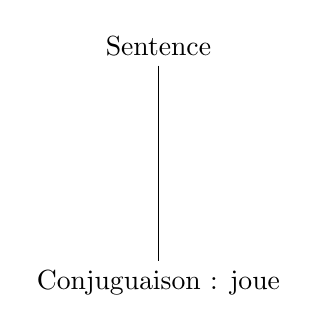
\begin{tikzpicture}
\node{Sentence}[sibling distance = 3cm, level distance = 3cm, align=center]
child {node {Conjuguaison : joue}};
\end{tikzpicture}
\end{center}
\end{document}
